    % Tony Mason (fsgeek@cs.ubc.ca)
%
% TEMPLATE for Usenix papers, specifically to meet requirements of USENIX '05
% originally a template for producing IEEE-format articles using LaTeX.
%
% written by Matthew Ward, CS Department, Worcester Polytechnic Institute.
% adapted by David Beazley for his excellent SWIG paper in Proceedings,  Tcl 96
% turned into a smartass generic template by De Clarke, with thanks to both 
% the above pioneers
%
% use at your own risk.  Complaints to /dev/null.
% make it two column with no page numbering, default is 10 point

% Munged by Fred Douglis <douglis@research.att.com> 10/97 to separate
% the .sty file from the LaTeX source template, so that people can
% more easily include the .sty file into an existing document.  Also
% changed to more closely follow the style guidelines as represented
% by the Word sample file. 

% Note that since 2010, USENIX does not require endnotes. If you want
% foot of page notes, don't include the endnotes package in the 
% usepackage command, below.

% This version uses the latex2e styles, not the very ancient 2.09 stuff.
\documentclass[letterpaper,twocolumn,10pt]{article}
\usepackage{usenix,epsfig,endnotes,textcomp}
\usepackage{hyperref}

% TM - I added these packages to allow highlighting so "to do" items can stand
% out and don't get forgotten.
\usepackage{xcolor,soul}
\usepackage{authblk}
\usepackage{balance}

\usepackage{upgreek}
\usepackage{comment}

\usepackage{geometry}

\usepackage{tikz}
\usetikzlibrary{calc}

% GanttHeader setups some parameters for the rest of the diagram
% #1 Width of the diagram
% #2 Width of the space reserved for task numbers
% #3 Width of the space reserved for task names
% #4 Number of months in the diagram
% In addition to these parameters, the layout of the diagram is influenced
% by keys defined below, such as y, which changes the vertical scale
\def\GanttHeader#1#2#3#4{%
 \pgfmathparse{(#1-#2-#3)/#4}
 \tikzset{y=7mm, task number/.style={left, font=\bfseries},
     task description/.style={text width=#3,  right, draw=none,
           font=\sffamily, xshift=#2,
           minimum height=2em},
     gantt bar/.style={draw=black, fill=blue!30},
     help lines/.style={draw=black!30, dashed},
     x=\pgfmathresult pt
     }
  \def\totalmonths{#4}
  \node (Header) [task description] at (0,0) {\textbf{\large Task Description}};
  \begin{scope}[shift=($(Header.south east)$)]
    \foreach \x in {1,...,#4}
      \node[above] at (\x,0) {\footnotesize\x};
 \end{scope}
}

% This macro adds a task to the diagram
% #1 Number of the task
% #2 Task's name
% #3 Starting date of the task (month's number, can be non-integer)
% #4 Task's duration in months (can be non-integer)
\def\Task#1#2#3#4{%
\node[task number] at ($(Header.west) + (0, -#1)$) {#1};
\node[task description] at (0,-#1) {#2};
\begin{scope}[shift=($(Header.south east)$)]
  \draw (0,-#1) rectangle +(\totalmonths, 1);
  \foreach \x in {1,...,\totalmonths}
    \draw[help lines] (\x,-#1) -- +(0,1);
  \filldraw[gantt bar] ($(#3, -#1+0.2)$) rectangle +(#4,0.6);
\end{scope}
}

\begin{document}

%make title bold and 14 pt font (Latex default is non-bold, 16 pt)
\title{PERC: Persistent, Efficient, Recoverable, Consistent \\
       Research Proficience Evaluation Proposal
}
% \titlenote{Produces the permission block, and copyright information}
% \subtitle{Utilizing Non-volatile Dual Inline Memory Modules}

%for single author (just remove % characters)
%\author{
%{\rm Tony Mason}\qquad
%{\rm Jake Wires}\qquad
%{\rm Andrew Warfield}\\
%{\rm fsgeek@cs.ubc.ca}\qquad
%{\rm jtwires@cs.ubc.ca}\qquad
%{\rm andy@cs.ubc.ca}\\
%Department of Computer Science, University of British Columbia, Vancouver, Canada
%} % end author

\author{Tony Mason\thanks{fsgeek@cs.ubc.ca}}
%\author{Jake Wires\thanks{jtwires@cs.ubc.ca}}
%\author{Andrew Warfield\thanks{andy@cs.ubc.ca}}
\affil{Department of Computer Science, University of British Columbia}

% suppress printing date
\date{}

\maketitle

\begin{abstract}
    This is a research proposal focused on advancing my research area and satisfy the \textbf{Research Proficiency Evaluation}, which is a
    qualifying requirement for the PhD program in Computer Science at the University of British Columbia.

    PERC is a study of the interactions of persistence and durability with respect to the application of byte-addressable non-volatile memory
    (\textbf{NVM}) when added to high performance key-value stores (\textbf{KVS}).  The issues to be explored include specifying a clear behavior
    model for NVM, with an emphasis on the class of failures that are anticipated and must be handled for \textit{crash consistency}, evaluating
    the changes that must be made to accomodate various durability guarantees (write, explicit sync, epoch) and the impact of those changes upon
    performance of existing KVS.   The expectation is that the work will provide greater insight into the trade-offs in the various approaches.
\end{abstract}

\section{Committee}

The following individuals have graciously agreed to serve as my committee for the purposes
of the Research Proficiency Evaluation:

\begin{tabular}{ll}
    Norm Hutchinson \\
    Alexandra Fedorova \\
    Andrew Warfield 
\end{tabular}

\section{Introduction}

Byte-addressable Non-volatile memory (\textbf{NVM}) that is directly connected to the memory bus, such as \textbf{NVDIMM-P} has been anticipated for many years but is just now emerging as actual, usable hardware.  Prior NVM solutions have consisted of either \textit{Block addressable non-volatile Memory} --- typically flash, or battery backed up DRAM with block addressable non-volatile memory for persistent storage.  These prior NVM solutions do not behave like directly accessed NVDIMM.

There is a body of existing work that suggests how NVM can be used to improve performance of performance-sensitive usages, including work done via a simulator.  However, this work suffers from weaknesses including: a lack of actual hardware and a na{\"i}ve model for failure.  Understanding NVM and how to correctly and efficiently use it will be important as we begin integrating it into critical systems infrastructure.

In this work, I propose analyzing the behavior of real systems that include NVM in order to understand the operational characteristics of that memory, identify a workable model for failure analysis that is consistent with the available information, identify potential ways in which NVM can be utilized to provide persistence, efficiency, recoverability, and consistency, and evaluate the tradeoffs inherent in integrating NVM into performance critical software.

\section{Background}

The motivation for this proposal is based upon my general research area.  The RPE supplement describes my original
broad research direction.  The exploration of that research direction has led to this current proposal. Since
that time I have been exploring more specific areas, with an eye towards refining my understanding of the research
area.  The initial work was an exploration in the general issues around extending file system functionality; this
resulted in the Finesse project, which evaluated using FUSE as an extensibility tool, by combining support for the
existing VFS interface with a non-system call approach that utilizes message passing to access new functional
interfaces.  That work was successful in demonstrating the ability to extend the interface, but was not persuasive.
Initial external feedback sees merit in the idea, but noted it is not sufficiently mature.

There are a number of challenges to the Finesse approach:

\begin {comment}

Sasha's comment:

You begin discussing drawbacks of Finesse, but you haven’t given the reader enough background about it. If
the proposal is not about Finesse, why include it? If there is a reason, state it, so the reader knows why
he or she is reading about it.

\end{comment}

\begin{itemize}
    \item FUSE has no ``pass-through'' mechanism (e.g., \textbf{ioctl}).
    \item Message passing on Linux is restrictive.  Existing mechanisms are viable, but severely limited
    (e.g., POSIX message queues) and require that we do considerable work to add functionality via this mechanism.
    \item Despite the vast number of FUSE file systems in existence, most are limited and not easily extensible.
    \item FUSE is itself not particularly well engineered for adding a dynamic extensibility model.
\end{itemize}

There are certainly a number of research opportunities within the FUSE area.  However, this does not further
my origianl research goal.  While I am not adverse to a change in direction, doing so requires a compelling
reason to do so.  Thus far, I have not found a persuasive argument to do so; I prefer to think this is due to
discipline rather than stubbornness.

\begin{comment}
Sasha's comment: 

Looks like you are trying to define a problem, but you have not defined it clearly enough. Provide examples,
measurements or other evidence as to why hierarchical file systems are bad for users. 

\end{comment}

Directly related to the original research area, I have been mulling over various models of data representation
and engaging in ``thought experiments'' in which I considered what a file system that supports semantics might
do.  In early April I spoke with another PhD student in the deparment, Francesco Vitale, who is doing research
in HCI.  His research area is personal digital data; I tend to think of this as data that is created based upon
an individual's own actions.  Thus, it would be distinguished from automatically created log data, for example.
He provided me with a number of HCI references that strongly support my concern about hierarchical file systems
not meshing well --- in essence, users's have been trained to implement their own organizational models for
their data within the interface provided \textit{despite} the clear case that it is not a good fit.  The HCI
community is constrained by what they can actually do within the existing systems model.  It is useful to note
that this type of data relationship modeling is not a single system problem; if anything, the problem becomes
vastly more interesting when we look at it as one that must cross system boundaries.  User data is not generally
limited to a single system.  I do not know what the model looks like right now, but a general model that
enables creating general, cross-realm relationships is critical for such an approach to be broadly useful.

Thus, my present thinking about how to approach the broader problem: I need to have a more flexible file system
that permits me to work with the HCI community to model different ways of creating data attributes.  The approach
I am currently considering is to model data as a \textit{graph}.  The model then is one in which we have files
(vertices) and relationships (edges).  This permits a mapping of the traditional hierarchical file system onto
such a graph.  There is a rather small body of work for graph file systems in existence; most of the work is
graph databases.

\begin{comment}
    Sasha's comment: 

    You have not motivated why representing files as a graph is a good idea, who needs this and what problem
    this idea solves. 
\end{comment}

A common approach to implementing graph databases is to utilize a key-value store (\textbf{KVS}).  This
observation piqued my curiosity about KVS. There has been tremendous interest in KVS recently, with a
half-dozen major systems papers on this topic over the past twelve months.  Thus, there is
a broad base of interesting information on constructing a KVS.

One area of KVS that has not been as well explored is their intersection with byte-addressable
non-volatile memory (\textbf{NVM}).  When I first started working with Andy, the area of interest was in
using NVM as a mechanism for acellerating file systems operations by optimizing the write path (validate,
log, return). It was this work that ultimately led me to the Finesse work; essentially all of my prior file
systems work has been \textit{in-kernel} on both UNIX and Windows (but not Linux).

The original design of that project (``Intentions'') involved a key-value store as well, with the intention
that it would be able to utilize NVM as it became available.  Hence, returning to this area for consideration
of this project was logical in terms of the flow of areas that I have been researching for over a year now.

\begin{figure*}
    \centering
    \caption{Sapience File Systems Project}\label{sapience}
    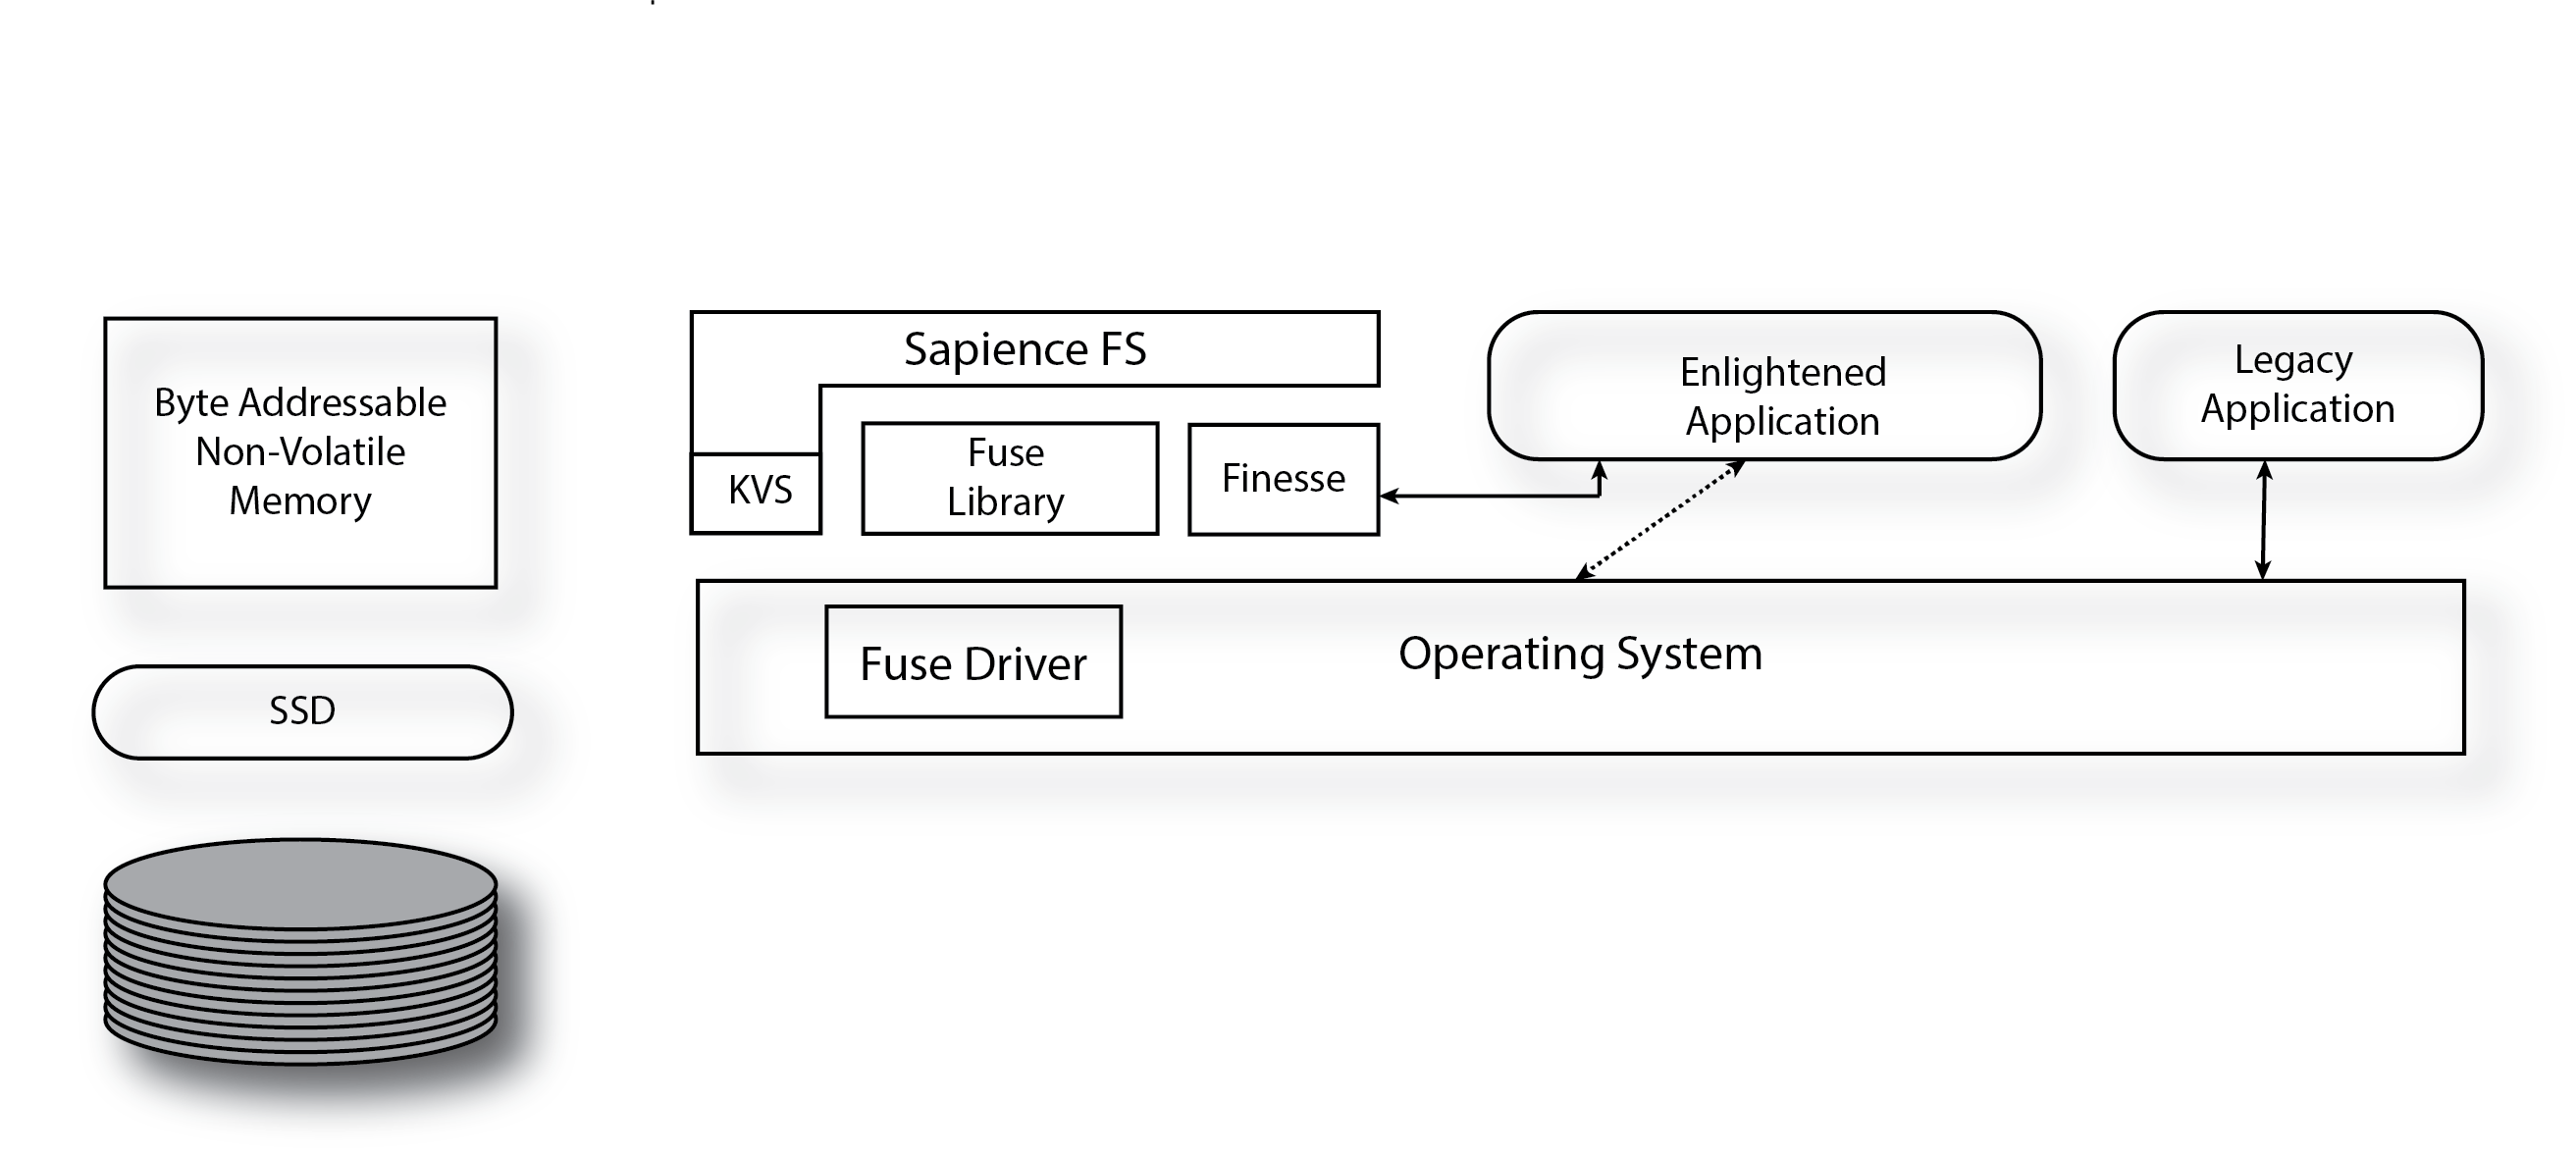
\includegraphics[width=0.45\textwidth]{figures/sapience.png}
\end{figure*}

Thus, the ``bigger picture'' for this project is that by constructing a key-value store, I have a natural basis
upon which to explore the Finesse-style extensions.  For example, adding a traditional key-value interface would
be one logical extension.  Another might be to explore a model in which the file system is itself implemented
in a distributed fashion --- an area that I discussed with Andy at one point --- so that different nodes could
each take a delegated region of the file system to manage.  This would look very much like a distributed file
system on a single system.

Another area to explore is an optimized IPC mechanism.  I have taken inspiration from the recent work on delegation
at SOSP 2017.~\cite{roghanchi2017ffwd} Combining this with a shared memory IPC mechanism could definitely provide
a useful improvement to the project as well as be useful for some of the other work envisioned.

\section{Proposal}

\begin{comment}
    Sasha's comment: 

    You described at length how your thinking evolved. Generally this is not what you include in systems papers. You are expected to present ideas and motivation. Most reviewers don’t care to learn how your thinking process evolved, though this might be interesting for an article on history of science. 
\end{comment}

\begin{comment}
From Andy 2018 May 01:

    Looks fine, probably a bit big for an RPE but I'm sure you are up for it.
    
    Goals is better than deliverables.  Deliverables could be restated in a few sentences.  Goals could be clearer -- an ideal version of that section is 3 short statements that can be evaluated as binary values in the end report -- as in, did you answer this question or not.  So coming up with consistency/durability models is a bit to vague because it sounds like there is a bunch of research you need to do to understand what's possible.  Can you scope it back to something more concrete and short term that is a step toward a paper and not a whole paper on it's own?
    
    Remember, the goal of the RPE is really to allow people who do not have the patience, tenacity, attention span, creativity, pain threshold, lack of better and more interesting hobbies and interests, or emotional fortitude to do research to self identify ahead of the full blow of failing after nine years of a phd.  It's not about identifying people who are good at research. ;)
    
    Some comments from tim harris on the persistent KV stuff:
    ---
    Here’s the memcached work I mentioned yesterday –
    
    https://timharris.uk/papers/2017-hotstorage.pdf
    https://timharris.uk/papers/2018-pmem.pdf
    
    My main take away was how difficult it was to move existing code to use byte-addressable NVM for heap storage.  With hindsight perhaps this should not have been a surprise.

My response 2018 May 01:

    Thanks for the feedback.  It mirrors some of my own concerns and actually reflects the size of the problem space and honestly that some of the ideas I have are not really fully baked; I wouldn’t even call them half-baked.  More like batter…
    
    The literature is clear (and it is consistent with my own experience): fences are bad.  The second paper you linked (which I have read and found interesting, particularly because it disagrees with another paper also published earlier this year) makes this point quite clearly – they are able to get down to one fence per transaction.  I’d like to find a way to get below that.  I have some ideas on how to do this, but I don’t have any actual work to back it up yet.
    
    Much of this will relate to the workload.  If there are many simultaneous requests, the logical thing to do is to simply stall sending responses until you can batch them together – the cache is going to naturally tend to push the data out anyway.  So doing a series of operations and flushing the cache line when you’re done with it but not fencing it makes a lot of sense.   Until that fence completes, though, you don’t have any guarantee that it has been committed.  Thus, one thing that would be good to know is the answer to: “what is the probability that a cache line has been committed at some specific time after you did that flush”.
    
    One possible model is to perform the transaction and flush the cache lines, then look to see if there is more work to do.  If there is, do that work.  If there isn’t, do the fence.  If it’s been “too long” since you did the last fence, do another fence.  In either case, send the acknowledgements for all the operations that were in completed state at the time the fence was started.  Then you can get less than once fence per transaction.  The “cost” for this is that the client waiting for the response will have to wait longer, so they see higher latency in the responses.  The win is that you use the system much more efficiently.
    
    I suspect, but do not know, that there are other interesting approaches available as well.  I’m pretty sure I’ve thought about and discarded several.  It seems likely that they will re-emerge at some point through this process
    
    Thus, I do actually view this as more of a research project.  Based upon your observation that the purpose of this isn’t to demonstrate research ability but to help the people that don’t have what it takes to self select out, perhaps that’s the wrong way for me to look at this.  I just didn’t like viewing this as a checkbox item. 
    
    I also have the first paper you linked but I don’t think I’ve read it yet, despite my sense that I’ve read dozens of papers.  I’ve printed it and will read it as well.
    
    If you don’t mind taking payment in sourdough bread, I’m fine with paying you. 😉  Is the cost higher if you provide feedback than if you just read them?
    
    I’ll mull over what you’ve said and make further revisions.  Part of what pushed me to send this out is that I am at the point where I need to start building something so I can trial some of the ideas that I’ve been mumbling to myself about for the past couple of months.
    
    Again, thanks much for the feedback.

From Andy 2018 May 02:

    Regarding fence/flush.  I like that you are thinking about partial approaches.  I'd encourage you to try to wrap some metrics around it.  When you are doing file system performance, I find things always go better when you start to measure request amplification from an outer syscall-level operation (e.g. pread) to the number of resulting IOs that you incur on the fastest and slowest paths.  Seems like you can do the same thing here in terms of characterizing the flush/fence impact.  This is in line with your proposal to build it and see if you need to do more... i'm just suggesting that you see if you can approximate what you expect up front, and reason about what the relationship is between your requests and your data structures that is going to have a structural impact on overhead.

In terms of other strategies, of course there are a bunch.  I suspect that at the end of the day this is going to come around to getting comfortable with some amount of inconsistency.  That's how you remove the barriers.  So down one path you have the versioned data structure / RCU thing that we discussed last time.  You can inconsistently write a whole bunch of new stuff, but you need to atomically map it in, and that atomic mapping carries a dependency that all the related updates (the new version) is also consistent.  The BetRFS b-epsilon tree has a related idea in this space which is that you put a journal at every node in the tree and accumulate writes in those, pushing them down as they fill.  This at least gives you batching and localization of the memory that you have to barrier on.

Regarding sourdough: I'm trying to cut carbs.  So that's kind of diabolical.  But to be clear: you get feedback either way -- the cost is for actually reading it first. :-P

\end{comment}

For this project, I choose to focus on one aspect of the larger research area.  One motivation for this is to ensure that it constitutes a research
area that I can undertake for a moderate period of time (four months) that will yield quantifiable research progress.  I note that beyond satisfying
the UBC RPE requirement, I hope to obtain work that can be incorporated into a useful research contribution in the form of a research paper for
submission.  My initial target would be the EuroSys conference deadline in late October, though NSDI (late September) is another possibility.  A
paper submission is not a requirement for the RPE; the paper may include additional work beyond that done for the RPE.

\textbf{This is a research proposal and as such is subject to revision during the lifetime of the research}.
It has been written based upon a broad survey of the literature --- a literature base that is under
considerable ``churn'' at the present time.  For example, in earlier iterations of this work I was
more interested in key-value stores.  In the period October 2018 to June 2018 there are multiple substantial
contributions in this area, including Anna (\S \ref{anna}), KV-Direct~\cite{Li:2017:KHI:3132747.3132756}, 
Faster~\cite{chandramouli2018Faster}, and Nibble~\cite{merritt2017concurrent}.

Similarly, the imminent availability of NVM hardware has created a bit of a frenzy of papers evaluating how
it can be integrated into existing systems.  This includes clfB-tree~\cite{kim2018clfb}, Efficient Logging in 
NVM~\cite{Cohen:2017:ELN:3152284.3133891}, UDORN~\cite{chen2017udorn}, Continuous Checkpointing~\cite{giles2017continuous},
NVHT~\cite{zhou2016nvht}, WHISPER~\cite{Nalli:2017:APM:3093337.3037730}, Persistent Lock-Free Queue for NVM~\cite{Friedman:2018:PLQ:3178487.3178490},
and Persistent Memory Transactions~\cite{marathe2018persistent}.

In doing this evaluation, I noted that much of the work assumes that cache line writes are \textbf{guaranteed} in the presence of a power failure.
WHISPER, for example, references an article on \url{lwn.net} that purportedly guarantees that this is the case.  When I followed up on that citation
it referenced an Intel source that ``recommended'' platform vendors correct for this. A slide deck presented several years ago by an Intel Fellow
in fact says that it is up to the platform vendor to provide this functionality.  I did find a SuperMicro patent filing that includes additional
\textbf{Memory Type Range Registers} that they proposed for this very purpose.

Even if they guarantee no cache-line tearing, there are no guarantees that any data structures more than a single cache line long would be properly preserved.  The Oracle work~\cite{marathe2018persistent} explicitly chooses to use checksums, while one of the other works [TBD] suggests using an alternating bit for detecting tears.

Thus, I would argue that the existing failure models are overly optimistic.  A model in which such failures can be detected and handled would be useful.
Analysis of that could form an element of a useful contribution in this area.  Even if the hardware can handle this for a single cache line, the need
to protect multiple cache line operations or dependencies seems prudent.

The existing mechanisms for consistency are simplistic and tend to utilize fencing fairly aggressively.  The prior literature also seems to converge around \textit{Epoch Consistency}, which if properly applied should require only a single store fence per epoch.

\begin{comment}

    Sasha's comment:

    Don’t expect that your reader will know what Jeff Dean numbers are. Or who Jeff Dean is. The chair of the exam may be from outside of systems area. 

\end{comment}

One aspect of analysis that seems to be missing from the prior work is an actual evaluation of the costs of various operations.  I have had the ``Jeff 
Dean'' numbers in my head for quite some time, but decided that nine year old performance numbers were probably not entirely accurate.  Tracking down 
this data confirmed this suspicion (and took some digging to find).  Current high-speed DDR-4 memory has a read latency of approximately 15 nanoseconds, 
and 25 nanoseconds for write operations (source is a publication by Crucial discussing clock cycles versus actual latency.~\cite{crucial2017latency}).

More broadly, understanding the costs of contention, such as on a spin lock, between threads of the same core as well as cores of the same CPU or cores on separate CPUs may be helpful in reasoning about synchronization trade-offs. 

This dovetails into this next point: another interesting line of inquiry is to evaluate the possibility of finding a \textit{hybrid} model for
data management.  For example, prior work
looks at delegation.~\cite{roghanchi2017ffwd,calciu2013message}  One objection to high performance shared nothing models is they do not perform well
when the workload becomes mixed.  Rather than abandon shared nothing, it might make more sense to have an adaptive model for switching from delegation
(shared nothing) to synchronized (synchronization).  Existing work takes an ``either/or'' position on these, when it seems clear they actually have
strengths in different scenarios.  Thus, a system in which we switch from one to the other might make better sense from a scaling perspective.  This
is a fairly open-ended research area and may be beyond the scope of a short research project area.  I keep it in mind because it may provide useful
performance insights.

\subsection{Goals}

\begin{comment}
    Sasha's comment:

    What does this line of inquiry have to do with NVDIMM?
\end{comment}

The goals for this proposal are to evaluate the performance trade-offs between performance and persistence, as realized by augmenting existing KVS.  To do this
effectively, the project must:

\begin{itemize}
    \item \textbf{Describe a Failure Model} --- in order to reason about crash consistency, it is important to have a clearly defined failure model.  In turn, this
    allows me to specify how crash consistency is guaranteed, relative to the failure model.  At a minimum, evaluating a cache-tearing model, versus atomic cache
    write-back model, will be evaluated.

    \item \textbf{Evaluate durability} --- there is an inherent trade-off between durability and performance.  At a minimum, my work must consider write-durability.
    In addition, I propose to also investigate other models, including fast-write (no durability guarantee), fsync (explicit durability), and epoch durability.
    For write-durability, aggressive flush versus block until completion will be evaluated.

    \item \textbf{Performance Evaluation} --- using at least two existing KVS, evaluate the impact of adding NVM durability to those systems.  Evaluation shall
    be both in terms of software impact (``how extensive are the changes?'') as well as benchmark impact.

\end{itemize}

The choice of KVS to use for this work will be part of the work itself.  At the present time, I would suggest considering choosing from MassTree,
Anna, Faster, and Nibble.  It may make the most sense to pick at least two that have been previously evaluated using the same benchmarks.  
Choosing implementations that have used different benchmarks may make it more difficult to compare to the prior published work.

The specific failure model needs to identify the particular problems that need to be considered.  This includes: using volatile addresses in
non-volatile memory, validating that for each intermediate state there is a clear mechanism for restoring consistency across a crash, ensuring we can
handle out-of-order write-back, and torn writes.  For example, something in the CPU cache may be evicted in an order that differs from the order in which 
it was written into the cache, which can change the temporal ordering.  A torn write occurs when only part of a cache line is written, such as in a power 
failure scenario.  Given that much of the prior work assumes no cache line tearing, it would be useful to measure the costs associated with that (e.g., 
checksumming, which currently has a cost of just over one CPU clock cycle per byte if using the Intel optimized CRC-32 algorithm.)

Durability relates to the guarantees provided to the caller.  In a model where I am modifying only existing KVS it makes sense to conform to the 
guarantees of the existing systems; if I can identify specific alternatives that are useful, they could be evaluated but likely not in the scope
of this project.

The key to this work is performance.  Thus, I need to be convincing in the micro-implementations that I make (ergo, demonstrating that they have excellent performance) as
well as how they are implemented within the context of the existing KVS.  While it would be ideal if my final results were a library, that may compromise performance, which
suggests that I must determine if the approach needs to be optimized to the existing KVS.

The lack of availability to \textbf{NVM} is a potential challenge to this work.  While it would be ideal if I can gain access to it, that is not guaranteed.  Thus, part of this work will be to either use an existing simulation, or provide a simple simulation to mimic the behavior of NVM on an existing system.   This is a significant open area
that presents a challenge for this project.

I propose considering the following consistency mechanisms as part of this work:

\begin{itemize}
    \item \textbf{Versioning} --- in this mechanism multiple \textit{versions} of a data structure are maintained.  The benefit of this approach is
    that it is easy to reason about.  The downside is that it amplifies storage utilization.
    \item \textbf{Logging} --- in this mechanism we utilize a journaling technique (redo, undo, or both) to permit recoverable atomic updates to
    operations.  The upside to this is that it is broadly general.  The downside is that it is more complex and may increase the serialization (fencing) requirements.
    \item \textbf{Shadow Copying} --- in this mechanism we use a read-copy-update mechanism for propagating changes through related data structures in
    such a way that the final update also makes the change visible.
    \item \textbf{HTM} --- in this mechanism, we use hardware transactional memory for performing operations.  The upside to this is that HTM exploits
    the existing hardware cache mechanisms, which happens to be the area we are concerned about.  The downside to this is that HTM has substantial
    limitations to our ability to utilize it as it may not be present on many platforms and even when it is avaialble there are significant
    restrictions on its usefulness.
\end{itemize}

Realistically, a viable solution is likely to employ one or more of these techniques, as appropriate.

This work will explore some or all of the following:

\begin{itemize}
    \item What to measure
    \item The tradeoffs between the consistency mechanisms
    \item Which consisency mechanisms are appropriate for specific situations
    \item Are there any prospective hybridizations of consistency mechanisms that exploit characteristics of memory?
    \item Impact of persistent memory versus dynamic memory
    \item Effect of read versus write asymmetry
    \item Strong versus weak consistency guarantees (focused on API models)
    \item Cost/benefit of various approaches applied to specific use cases
    \item Provide a description of actions for each consistency mechanism ("what happens when")
    \item How to expose NVM to a container
\end{itemize}

Note that the initial analysis will be done with conventional dynamic memory and then consider how replacement with NVM changes the analysis.
What functionality becomes redundant?  What functionality is \textit{missing} or needs to be added in the new model.  How does it impact the tradeoffs and
how well does it address the needs for our systems?  How do we add any missing functionality?

My expectation is that to use NVM efficiently will involve investigating specific techniques that permit minimizing fence operations, such as 
\textit{batching}. For example, if the
interface guarantees that an update is persistent when the \textbf{put} operation is complete, I may be able to defer the put operation.  Thus,
for example, a rather straight-forward mechanism would be to fence if there is no more pending work to perform or if there is pending work to
perform and some time (the \textit{epoch} period) has not yet elapsed.  While this will increase the latency for a single operation, it should
yield a system that provides better overall throughput.

Another approach that may make sense (and could ultimately lead in a direction of buiding a new optimized KVS) is to provide a richer interface: one in which the operations may be asynchronous.  This permits higher levels to issue a series of calls and then either force a fence or ask for a return once
a specific epoch has been achieved.

\subsection{Deliverables}

The deliverables for this project are:

\begin{itemize}

    \item \textbf{Reference Curations} --- thus far I have done short (approximately 1000 works) curations for a number of the background papers
    in this work.  I intend on continuing to do this work.  I do not expect to curate all those papers, but there are a number of additional papers that are relevant and useful in understanding this work.  Thus, I will continue to do those write-ups as part of this project work.

    \item \textbf{Project Paper} --- the final outcome of this project should be a paper that summarizes the work that I did for this project, my
    findings, and my conclusions. It should be of sufficient detail that a reader can understand what I did and reproduce my results.

    \item \textbf{Presentation} --- a presentation of my work and findings, suitable for presentation to a general computer science audience
    to explain the project, my findings, and my conclusions.

    \item \textbf{Project Repository} --- a complete repository that includes any code I used for the project, data that I collected and
    produced during the project, the paper, and the presentation for the project.
\end{itemize}

The expectation is that I will officially present this in Fall 2018 at a data and time to be determined.

\subsection{Schedule}

The schedule for this project is shown in Figure \ref{schedule}

\begin{figure*}
    \centering
    \caption{Project Schedule by Week}\label{schedule}
    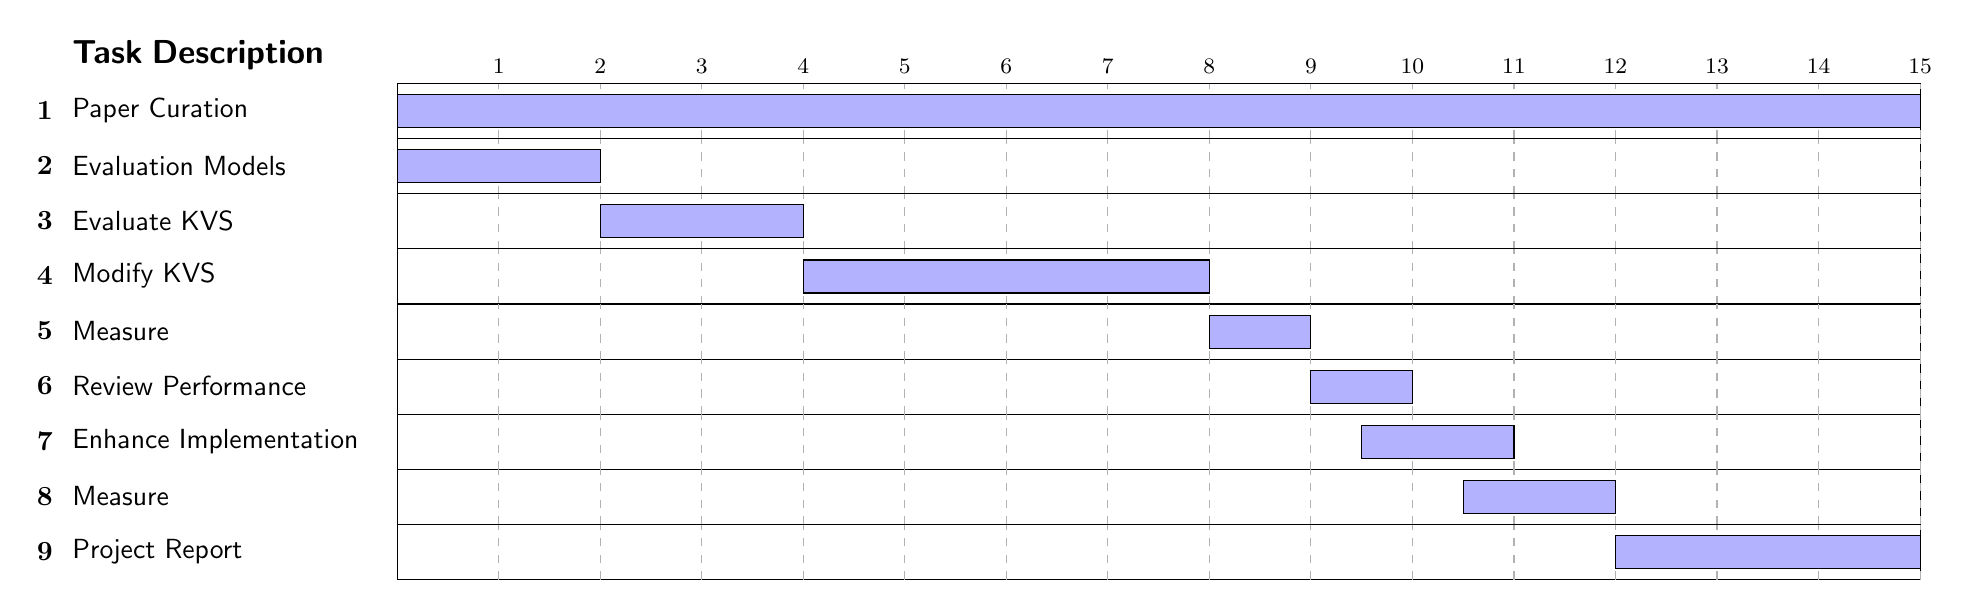
\begin{tikzpicture}
        \GanttHeader{1.95\columnwidth}{2ex}{4cm}{15}
        \Task{1}{Paper Curation}{0}{15}
        \Task{2}{Evaluation Models}{0}{2}
        \Task{3}{Evaluate KVS}{2}{2}
        \Task{4}{Modify KVS}{4}{4}
        \Task{5}{Measure}{8}{1}
        \Task{6}{Review Performance}{9}{1}
        \Task{7}{Enhance Implementation}{9.5}{1.5}
        \Task{8}{Measure}{10.5}{1.5}
        \Task{9}{Project Report}{12}{3}
    \end{tikzpicture}
\end{figure*}

In addition, the presentation of this work will be scheduled (to be determined) for Fall 2018.

\section{Supplement}

The supplemental material that was originally included with this document has been moved to a separate
document entitled \textit{PERC Supplementation Material}.


\newpage
\balance

{\footnotesize \bibliographystyle{acm}
\bibliography{nvdimm.bib,phd-app-ref.bib}}


% \theendnotes

\end{document}

